\section{Result 2}
With the ease at which the \textit{nETL} software handled loading data in Run 1, and the ease at which CouchDB was able to handle indexing, a second run was created with multiple courses. For this run, 40 courses were selected: ECO1010F, ECO1011S, ACC1006F, STA1000S, ECO2003F, BUS1036F, ECO2004S, CML1001F, MAM1010F, PSY1004F, FTX2024S, ECO2007S, ACC2011S, CSC1015F, PHI2043S, ACC3023S, INF2004F, PSY1005S, STA2020F, CML2010S, CML2001F, SOC1001F, ACC2018S, SOC1005S, BUS2010F, ACC2012W, AXL1100S, ACC3022H, ACC3004H, PHY1012F, MAM1020F, PHI2043F, FTX3045S, ACC3009W, MAM1012S, FTX3044F, MAM1000W, POL1004F, CSC1016S, ACC4000H. These courses were selected simply because they have a high level of student enrollment. \textit{nETL} filtering on the courseCode field was configured to allow all these codes. Filtering on student IDs in the demographic was removed, since over 10 000 student numbers would need to be included a list for such a filter.

Compared to Run1, there is a significant increase in the size footprint of the view index (from \textless 1MB to 143MB) do to the requirement of duplicating demographic output in the map function. Performance of the list function degraded considerably, with streaming of the 2MB CSV taking several minutes. To efficiently retrieve view output of larger indexes would require implementing data retrieval outside of CouchDB. List functions require iterating through every view output individually, whereas working with the view directly would allow for retrieving in batches which is much more efficient. \textit{nETL} could be configured to do this, but hasn't been.

todo: The map function is the same as used for result 1

\begin{figure}[ht]
    \centering
    \begin{mdframed}
        \centering
        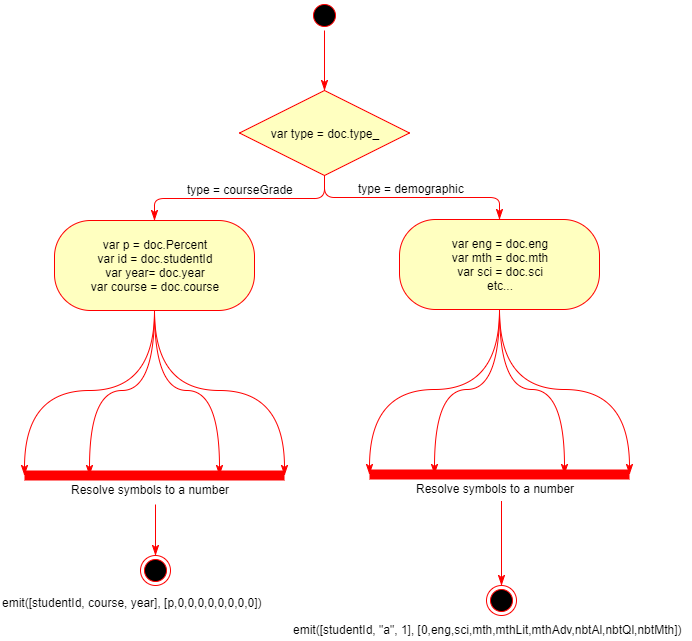
\includegraphics[scale=0.35]{./resources/figures/activity-diagram-1.png}
    \end{mdframed}
    \caption[Result 1 Map function]{\textbf{Figure \ref{result-1-map-fn}: Activity diagram showing logic Map function logic for Result 1.} }
    \label{result-1-map-fn}
\end{figure}

\subsection{Correlation analysis}
The results for \textit{Run 1} and \textit{Run 2} have been summarized in the graphs in Figure \ref{run1-chart1}; several courses were picked at random to show correlation between course grades and student benchmarks. The results show that in general, higher benchmarking scores are indicative of higher course results overall. Some of the benchmarks show stronger correlation to grade results than other, as seen by steeper trendline gradient.



\begin{figure}[H]
    \centering
    \begin{mdframed}
        \centering
        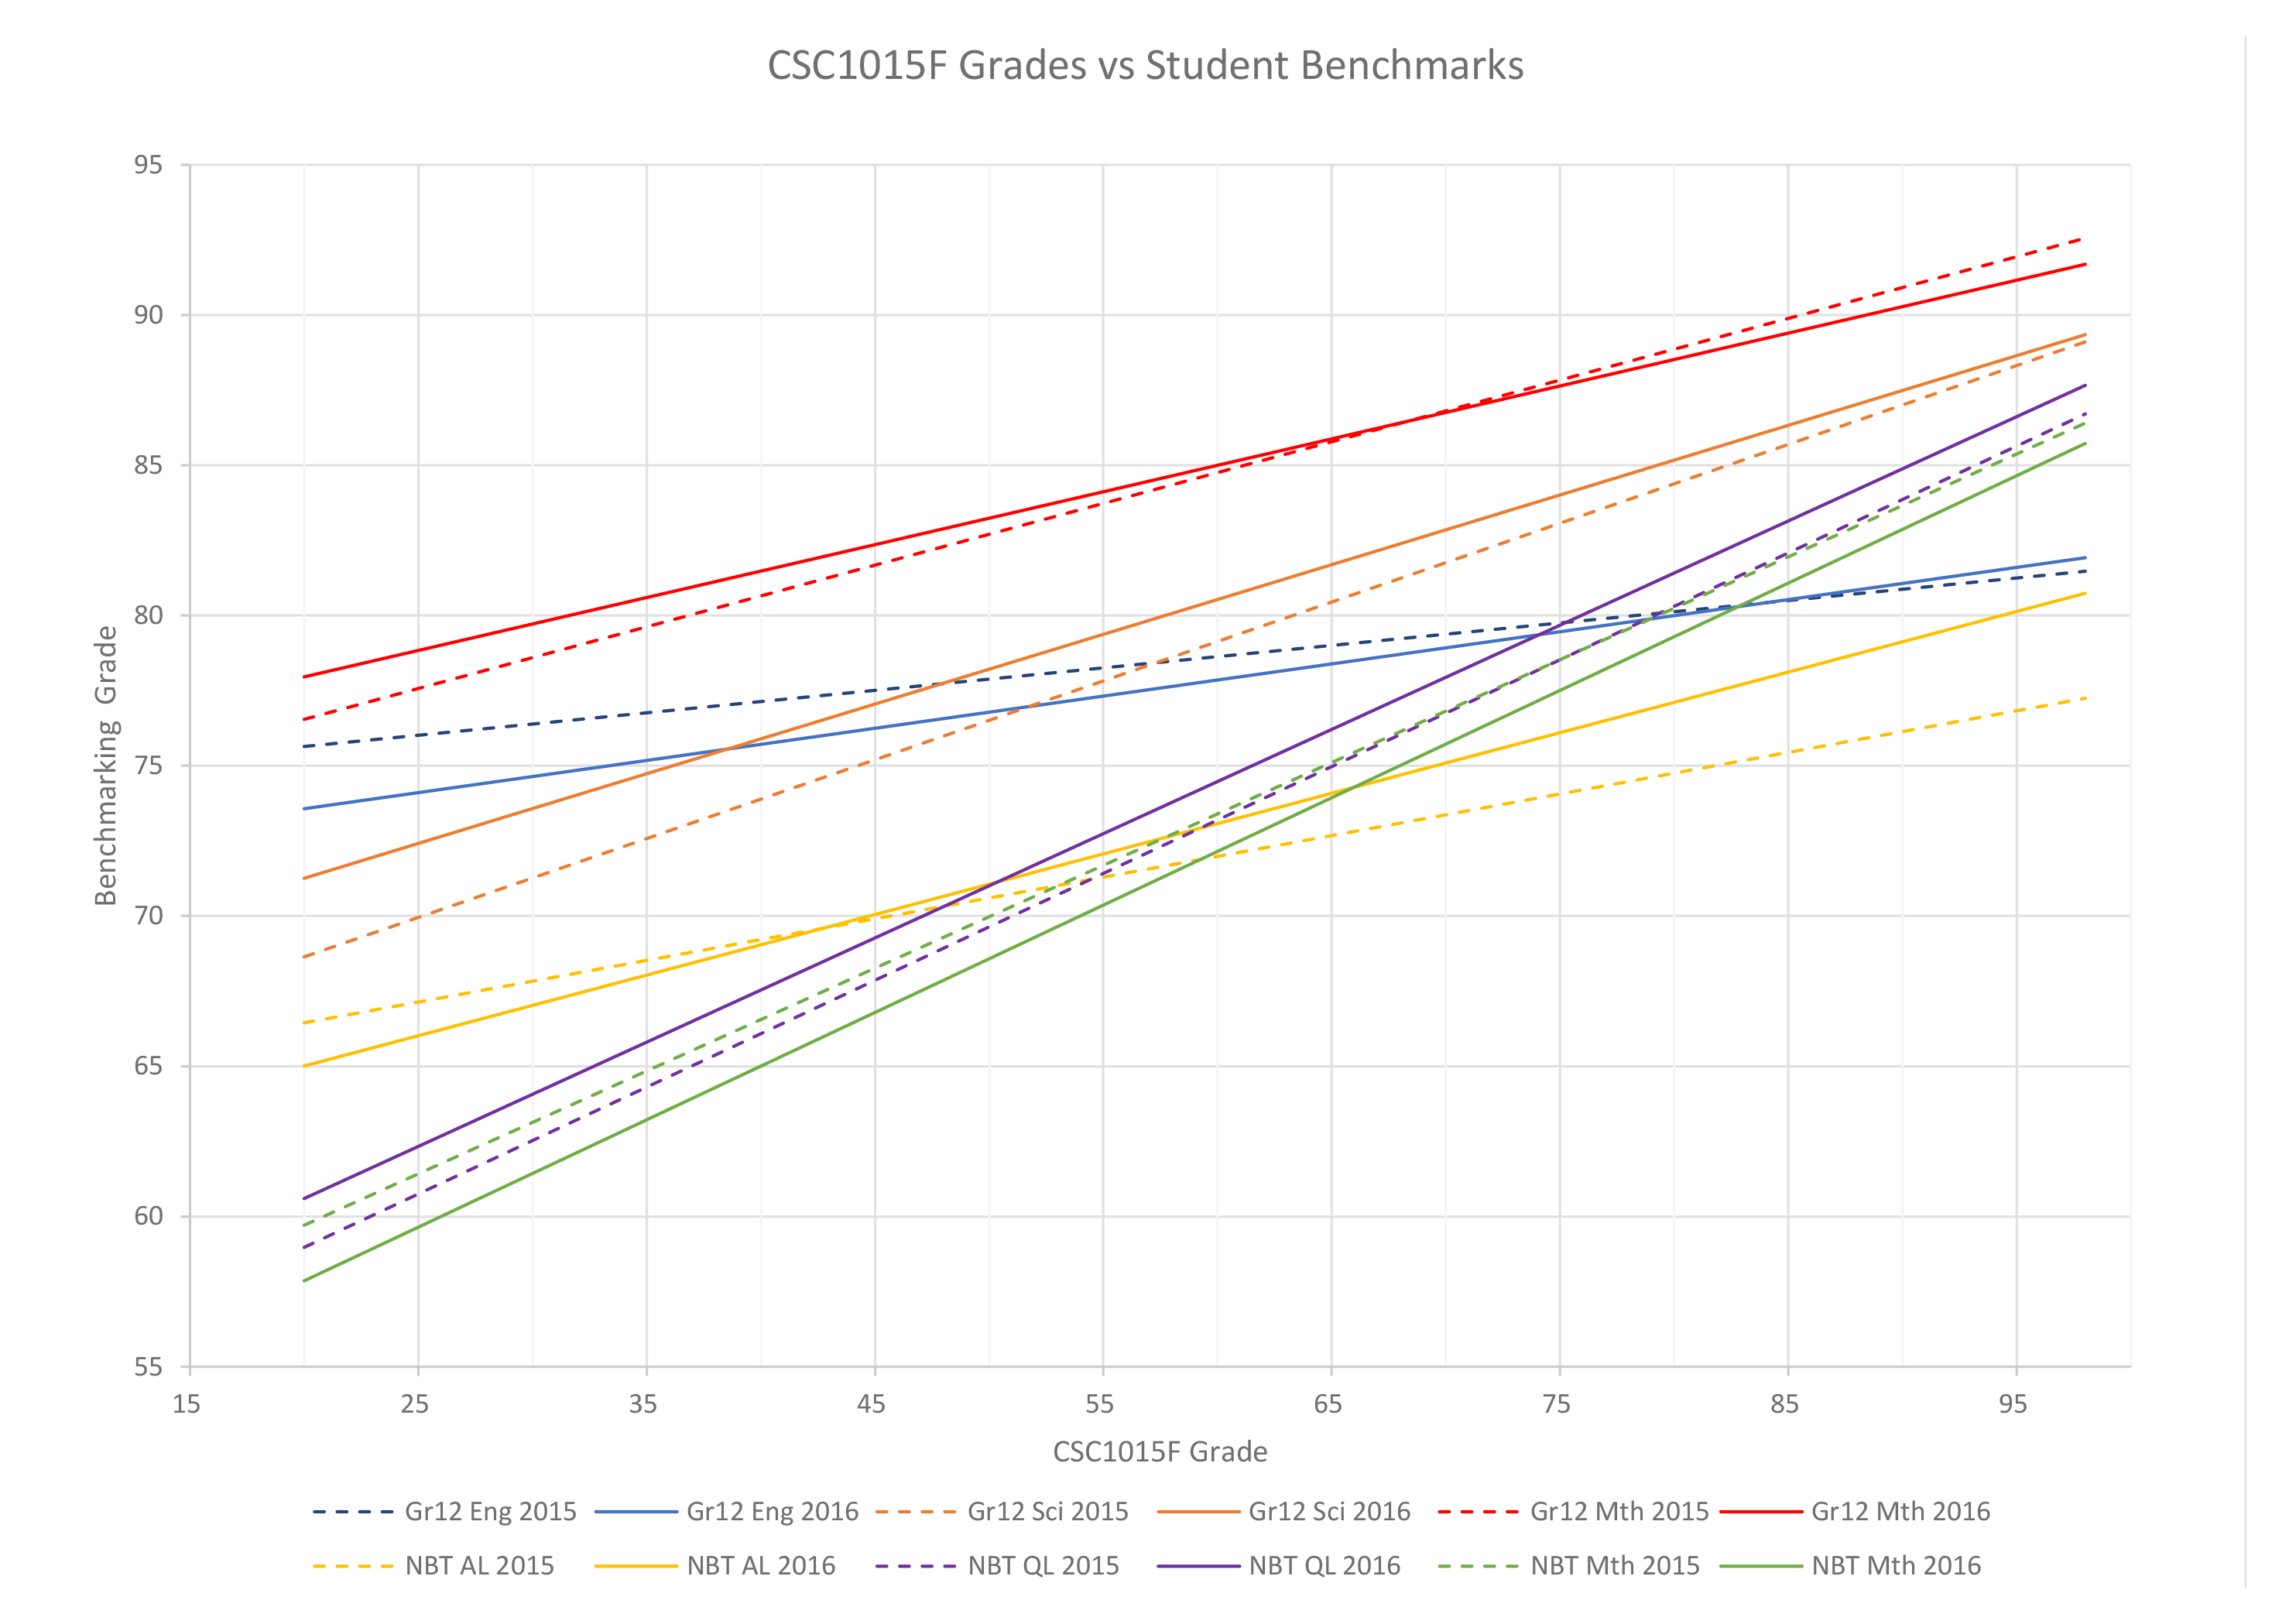
\includegraphics[scale=0.55]{./resources/figures/run1-chart1.png}
    \end{mdframed}
    \caption[CSC1015 grade vs benchmark correlation]{\textbf{Figure \ref{run1-chart1}: Correlation between student benchmarks and CSC1015F results.} This graph shows benchmark scores plotted against the final CSC1015F grade. Datasets focus on a single benchmark, so a trendline shows the correlation between a single benchmark and final grades.}
    \label{run1-chart1}
\end{figure}